% !TEX encoding = UTF-8 Unicode

\documentclass[a4paper]{article}

\usepackage{color}
\usepackage{float}
\usepackage{url}
\usepackage{listings}
\usepackage[T2A]{fontenc} % enable Cyrillic fonts
\usepackage[utf8]{inputenc} % make weird characters work
\usepackage{graphicx}
\usepackage{physics}

\usepackage[english,serbian]{babel}
%\usepackage[english,serbianc]{babel} %ukljuciti babel sa ovim opcijama, umesto gornjim, ukoliko se koristi cirilica

\usepackage[unicode]{hyperref}
\hypersetup{colorlinks,citecolor=green,filecolor=green,linkcolor=blue,urlcolor=blue}

%\newtheorem{primer}{Пример}[section] %ćirilični primer
\newtheorem{primer}{Primer}[section]

\begin{document}

\title{Uvod u kvantno računarstvo sa osvrtom na funkcionalne programske jezike za kvantno programiranje\\ \small{Seminarski rad u okviru kursa\\Metodologija stručnog i naučnog rada\\ Matematički fakultet}}

\author{Aleksandar Ćurković, Nemanja Šekularac\\ curkovical@gmail.com, nemanja.sekularac@gmail.com}
\date{14.~april 2015.}
\maketitle

\abstract{
U ovom radu prikazujemo funkcionalne programske jezike za kvantno programiranje, uz kratak osvrt na osnove kvantnog računarstva i funkcionalne programske jezike uopšte.
Propratni primeri realizovani su u programskom jeziku Quipper.

\tableofcontents

\newpage

\section{Uvod}
\label{sec:uvod}

\subsection{Kvantno računarstvo}
\label{sec:kvantnoracunarstvo}

Kvantno računarstvo je oblast istraživanja koja se bavi računarskim sistemima koji u svom radu direktno koriste efekte kvantne mehanike.
Kvantni efekti, kao što su superpozicija (eng.~\em{superposition}) i kvantna zapletenost (eng. ~\em{quantum entanglement}) se u ovim sistemima, koje nazivamo kvantnim računarima tretiraju kao resurs i koriste za izvršavanje operacija nad podacima.

\subsection{Osnovni pojmovi kvantnog računarstva}

\subsubsection {Kubit}

Kubit (eng.~\emph{qubit, quantum bit}) je najmanja jedinica izračunavanja u kvantnom računarstvu.

Kubit je pandan jednom bitu informacija u klasičnom računarstvu, ali dok se jedan bit može naći u 2 diskretna stanja (0, 1),
kubit, na osnovu kvantnog principa superpozicije može istovremeno biti u oba.
Tačnije, stanje kubita, u odsustvu merenja, može biti bilo koja linearna kombinacija osnovnih stanja.
Za osnovna stanja (eng. ~\em base states) kubita se uzimaju ona koja pri merenju prelaze u stanje 0 ili 1 sa verovatnoćom 1 i obeležavaju se sa $\ket{1}$ i $\ket{0}$

Formalno, stanje kubita se zapisuje kao $\alpha \ket{0} + \beta \ket{1}$ gde su $\alpha i \beta$ \em{kompleksni} parametri koji označavaju verovatnoću da se nakon merenja (očitavanja stanja) kubit nađe u jednom od osnovnih stanja sa verovatnoćama, redom, $\alpha^2$ i $\beta^2$ i važi $\alpha^2+\beta^2=1$

Ovo svojstvo ima za posledicu da se 2 kubita mogu naći istovremeno u 4 različita stanja i generalno, n kubita može odjednom biti u $2^n$ različitih stanja.

Skup kubita uzetih zajedno naziva se kvantni registar. (eng.~\emph{quantum register}).

\subsubsection{Zapletenost, kombinovanje kubita, kvantni paralelizam}
\label{entanglement}

Efekat kvantne zapletenosti se manifestuje visoko koreliranim stanjima zapletenih čestica nakon merenja.
To nam omogućava da kombinujemo kubite na način na koji to nije moguće sa bitovima. Stanje sistema od 2 zapletena kubita predstavlja se kao linearna kombinacija svih kombinacija osnovnih stanja oba elementa.\\

$\alpha\ket{00} + \beta\ket{01} + \gamma\ket{10} + \delta\ket{11}$\\

pri čemu su $\alpha^2, \beta^2, \gamma^2, \delta^2,$ redom verovatnoće da će se sistem naći u odgovarajućoj kombinaciji osnovnih stanja gde i dalje važi\\

$\alpha^2+\beta^2+\gamma^2+\delta^2=1$.\\

Ovakva distribucija verovatnoća naziva se \textit{pomešano stanje}\cite{qfc}. Svaki posmatrač može imati svoje pomešano (nekompletno) stanje, dok se stvarno stanje kvantnog sistema nalazi u (moguće nepoznatom) \textit{čistom stanju}.

Ovo nam omogućava da, u teoriji, funkcije na kvantnim računarima evaluiramo za više vrednosti \emph{odjednom} tako što vrednosti zadamo u terminima parametara zapletenog sistema. Ovaj efekat, kvantni paralelizam (eng.~\emph{quantum parallelism}) suštinski odvaja kvantno od klasičnog računarstva.

Nažalost, ovo funkcioniše samo dok je sistem u stanju koherencije  tj dok su superpozicija i spletenost očuvani.

\subsubsection {Operacije nad kubitima, kvantne kapije}

Zbog očuvanja koherencije sistema i informacija u toku izvršenja, sve operacije nad kubitima i sistemima kubita moraju biti reverzibilne (eng.~\emph{reversible}).

Formalno ove operacije predstavljamo unitarnim operatorima nad izabranim prostorom stanja sistema.

Kvantna logička kapija (eng. ~\emph{quantum logic gate}) je kvantni pandan logičkoj kapiji klasičnog računarstva i predstavlja jednu takvu operaciju.

Posebno su nam, kao i u klasičnom računarstvu, zanimljive male kvantne logičke kapije koje mogu da svojom kombinacijom predstavljaju druge operacije ( ili da ih barem proizvoljno približno aproksimiraju sa konačnim brojem osnovnih kapija). Jedan takav \emph{univerzalni set kapija} su na primer Hadamardova kapija (eng~\emph{Hadamard gate})\\
\smallskip
$H\equiv\frac{1}{\sqrt{2}}\begin{pmatrix}
1&1\\
-1&1
\end{pmatrix}$\\
\smallskip
koja radi nad jednim kubitom na sledeći način:\\
\smallskip
$\ket{0} \rightarrow \frac{1}{\sqrt{2}}(\ket{0} + \ket{1})$\\
\smallskip
$\ket{1} \rightarrow \frac{1}{\sqrt{2}}(\ket{0} - \ket{1})$\\

i Toffoli kapija (eng.~\emph{Toffoli gate}) (Toffoli je reverzibilna logička kapija u klasičnom računarstvu i može se predstaviti u kvantnom obliku).

Detaljnije informacije o osnovama kvantnog računarstva mogu se naći npr. u \cite{knjiga}

\subsubsection{Kvantno kolo, Kvantni algoritam, Modeli kvantnog računara}
\label{modeli}

Kvantno kolo je sekvenca kvantnih kapija kao osnovnih operacija koje vrše transformacije nad jednim ili više kubita. Samo kvantno kolo predstavlja jednu unitarnu operaciju (kao kombinacija unitarnih operacija/kapija)

Da bismo kvantno kolo upotrebili za izračunavanje potrebno je sistem na koji je primenjeno najpre inicijalizovati na nek početne vrednosti.

Da bi smo rezultat izračunavanja vratili u klasični računar potrebno nam je merenje. U kvantnoj mehanici merenje je nereverzibilna, destruktivna operacija koja sistem dovodi u stanje dekoherencije.

Takođe merenje je probabilistička operacija (kvantni računari dele osobine sa probabilističkim i nedeterminističkim računarima i rešenje daju samo sa određenom tačnošću).

To dovodi do toga da je opšti upotrebljivi kvantni algoritam niz uzastopnih inicijalizacija, primenjenih kvantnih kola i merenja sa dodatim klasičnim operacijama (npr provere rezultata ili kontrole toka).

Praktična konstrukcija kvantnog računara je još uvek u domenu laboratorijskih eksperimenata uz tek poneki komercijalni pokušaj.

Za potrebe kvantnog računarstva, sisteme predstavljamo različitim idealizovanim modelima kao što su npr kvantna Turingova mašina (eng.~\emph{quantum Turing machine, QTM}) ili kvantno kolo (eng. ~\emph{quantum circuit}) dok zanemarujemo prisustvo greške i efekte smetnji (eng.~\emph{interference}) i dekoherencije koji su realnost kvantnih računara.

Neki od opisanih funkcionalnih jezika (Quipper, ?) rade na modelu kvantne memorije sa nasumičnim pristupom (eng.~\emph{Quantum Random Access Memory, Quantum RAM, QRAM} opisan u \cite{qram_model}

Kvantni računar je zamišljen kao koprocesor povezan sa klasičnim računarom na kome se izvršava kontrola toka. Kvantni uređaj sadrži fiksni unapred određeni broj kubita i sposoban je da ih individualno adresira. Na kvantnom računaru se izvršavaju samo 2 tipa operacija, unitarne operacije i merenja.  Smatra se da je određen broj osnovnih unitarnih operacija realizovan kroz ugrađenje kvantne kapije i da su one oblika ''Primeni ugrađenu operaciju na određene kubite''. Ove operacije vraćaju potvrdu kvantnog računara o izvršenju ali ne i bilo kakvu drugu informaciju.

Informacije o rezultatu se dobijaju operacijama merenja, oblika ''izmeri kubit q'', ova operacija vraća 0 ili 1 klasičnom računaru sa određenim verovatnoćama.

\subsection{Funkcionalno programiranje}
\label{sec:funkcionalniprgjezici}

Funkcionalno programiranje je programska paradigma u kojoj je osnovni način izračunavanja primena funkcija na argumente.\cite[p. 3]{funcPro}
Funkcionalni programski jezici su jezici koji podržavaju i ohrabruju primenu funkcionalne paradigme.
Tradicionalni programski jezici se baziraju na ideji promenljiva kao promenljive veze između imena i vrednosti. Ovi jezici se nazivaju 
imperativni jer se sastoje od niza komandi, koje čine dodele koje menjaju vrednost promenljive.
Funkcionalni jezici se baziraju na strukturiranim pozivima funkcija. Funkcionalni program se sastoji od poziva funkcije koja može da
poziva druge funkcije:\\
<function1>(<function2>(<function3> ... ) ... ))\cite[p. 4]{funcPro}

Među najbitnijim konceptima funkcionalnog programiranja su funkcije višeg reda i odsustvo nuspojava. \\
Funkcije višeg reda su funkcije koje ili mogu za argumente uzeti druge funkcije ili kao svoj rezultat vraćaju funkciju, čime se omogućavaju ugnježdeni pozivi funkcija, odn. pojava koje se zove kompozicija funkcija.\\
Eliminacija nuspojava podrazumeva otklanjanje svih promena koje ne zavise od pozvane funkcije i njenih argumenata, tako da više poziva jedne funkcije uvek vraća isti rezultat ako su argumenti poziva isti. Eliminacijom nuspojava olakšava se razumevanje programa i formalna 
verifikacija a redosled izvršavanja postaje nebitan.\par
Prvi i dugo vremena najpopularniji funkcionalni programski jezik je Lisp (LISt Processor) nastao 1958. pod uticajem lamda računa, ali 
zadržavajući dodelu vrednosti promenljivoj. Glavna struktura podataka u Lisp-u je povezana lista. Prvi čisti funkcionalni jezik 
(bez dodele vrednosti promenljivoj) je ISWIM. Još neki bitni funkcionalni jezici su Erlang, Haskell, ML, Scala, F\# itd.

\section{Funkcionalni programski jezici za kvantno programiranje}
\label{sec:funcprl_qp}
Kvantni funkcionalni jezici zasnivaju se na konceptu lambda računa. Lambda račun je formalni sistem u matematičkoj logici koji se koristi za ispitivanje svojstava funkcija, kao što su izračunljivost, rekurzija i zaustavljanje.\cite{survey} Među ove jezike spadaju: QFC, QML, Quantum lambda calculi i Quipper, od kojih ćemo malo detaljnije obraditi QFC (QPL) i Quipper.

\subsection{QFC i QPL}
\label{sec:qfc_qml}

QFC ( \emph{eng}. Quantum Flow Charts) i QPL ( \emph{eng}. Quantum Programming Language) su dva blisko povezana jezika čiji je tvorac Peter Selinger.  Pristup programiranju u njima se može sumirati na sledeci način: ''kvantni podaci, klasična kontrola'' \cite[p. 1]{qfc}. Postoje dva načina sintaksnog predstavljanja kvantnih programa: grafička reprezentacija, u vidu grafikona protoka, i tekstualna. Izbor između te dve sintakse je pitanje ukusa, jer su međusobno ekvivalentne. \cite[p. 2]{qfc} Dva osnovna načina manipulacije kubitovima: unitarne transformacije i merenja. Klasični kontroler komunicira sa kvantnim uređajem šaljući mu niz instrukcija koje kvantni računar zatim izvršava. 

Program se predstavlja u obliku grafikona protoka odn. dijagrama kontrole protoka. Komande deluju tako što ulaz transformišu u izlaz. Zarad jednostavnosti razmatramo samo jedan tip podataka: kubit. Ako nije drugačije naglašeno, tok podataka se odvija od vrha prema dnu. Svaka grana je označena kubitovima koji su dostupni u tom delu programa dok se u čvorovima odvijaju operacije nad njima. Unitarne transformacije mogu da deluju na jedan ili više kubitova; npr. pišemo \textit{q*=S} za operaciju primene neke kvantne logičke kapije na kubit q. Dakle, notacija je analogna notaciji \textit{b:=1} u klasičnom računarstvu. Operacija merenja je granajuća jer može imati dva moguća izlaza.
\begin{figure}[H]
\caption{Primer jednostavnog programa napisanog u QFC} \label{fig:qfcPrimer}
\centering
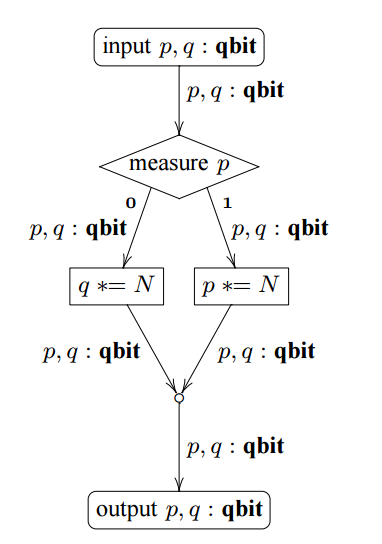
\includegraphics[scale=0.75]{qFlow}
\label{fig:qfcPrimer}
\end{figure}
Verovatno najbolje objašnjenje pruža razmotranje jednostavnog primera na slici 1: program prima dva kubita- \textit{p} i \textit{q}, meri p i onda primenjuje logičku kapiju Not na jedan od kubitova u zavisnosti od merenje \textit{p}. Na kraju, na izlazu vraća modifikovane kubitove p i q.

Primetimo da ako su ulazni kubitovi u čistom stanju, oni će to stanje zadržati posle svake unitarne transformacije i operacije merenja. Trenutak kada se to stanje menja je prilikom spajanja dve grane na dijagramu, tako da na izlazu (u ovom slučaju) dobijamo kubitove u pomešanom stanju. Ali i sam ulaz u program mogu biti kubitovi u pomešanom stanju u kom slučaju se logičke kapije primenjuju na matrice gustine koje predstavljaju pomešana stanja. Dok se čisto stanje može predstaviti u obliku matrice sa jednom kolonom, matrica gustine jednog kubita je dimenzije 2$\times$2. Npr., za kubit \textit{u}=$\frac{1}{\sqrt{2}}\ket{0}$ - $\frac{1}{\sqrt{2}}\ket{0}$ 
matrica gustine je \[\textit{uu*}= \left( \begin{array}{cc}
\frac{1}{2} & \frac{-1}{2} \\
\frac{-1}{2} & \frac{1}{2} \\
\end{array} \right).\cite[p.~11]{qfc}\]

Postoje još neka pravila kao što su: ''new'' koje alocira novu promenljivu i njenu vrednost postavlja na 0, ''discard'' koje dealocira promenljivu, ''initial'' koje označava početak novog (nedostupnog) toka kontrole i ''permute'' koje permutuje promenljive u trenutnom kontekstu promenljivih.

QFC podržava petlje (nastaju dodavanjem linije toka kontrole od jedne tačke do druge), procedure (nalik funkcijama u \emph{C}-u imaju ime, tip, ulazne argumente i povratnu vrednost) i rekurziju.

\subsubsection{Implementacioni detalji}

Iako kvantni hardver trenutno ne postoji, korisno je obratiti pažnju na nekoliko hipotetičkih detalja eventualnog hardverskog rešenja. Operativni sistem bi trebao da pamti listu kubitova koje koristi svaki od procesa. Kada proces zatraži novi kubit, operativni sistem nalazi slobodan kubit koji mu dodeljuje. Naravno, operativni sistem mora da vodi računa o tome da proces ne može da pristupi kubitu koji mu nije dodeljen, što veoma liči na upravljanje memorijom na klasičnim računarima. Kada proces završi rad sa nekim kubitom obaveštava o tome operativni sistem koji dati kubit označava kao slobodan.\cite[p. 21]{qfc}

Po \textit{svojstvu nekloniranja} nije moguće duplicirati kvantni bit. U ovom jeziku, koji je statično tipiziran, ta teorema je ispoštovana u samoj sintaksi, što predstavlja napredak u odnosu na ranije formalizme koji nisu imali to svojstvo, što bi kasnije dovelo do grešaka u radu (npr. prilikom primene unitarne transformacije na više kopija istog kubita).

\subsection{Quipper}
\label{sec:quipper}

Quipper je skalabilni (eng.~\emph{scalable}), ekspresivni, funkcionalni programski jezik višeg nivoa (eng.~ \emph{higher-order}).
Prvi put predstavljen 2013. godine u \cite{quipper_language}.

\subsubsection{Model}

Quipper kao model kvantnog računara koristi QRAM model kratko opisan u \ref{modeli}, detaljno u \cite{qram_model} 


\subsubsection{Odlike jezika}

Prošireni model kola - osim unitarnih kapija/kola quipper obezbeđuje ugrađenu podršku za eksplicitnu inicijalizaciju i prekid (eng.~\emph{termination}), merenja, klasične bitove, klasične kapije i klasično-kontrolisane kvantne kapije 

Pomoćni kubiti (eng.~\emph{ancilliary qubits, ancillas}) - dopunski ulazi koji su potrebni za neke kvantne algoritme (npr. pretpostavlja se da su u stanju $\ket{0}$ pre i posle izvršenja), eksplicitna inicijalizacija i prekid omogućavaju kontrolu opsega (eng.~\emph{scope})

Prekidanje sa potvrdom (eng.~\emph{assertive termination}) - operacija koja ''dealocira'' kubit uz potvrdu da je u stanju $\ket{0}$\\

Mešana klasično/kvantna kola - klasični bitovi, klasične kapije i klasično kontrolisane kvantne kapije se mogu slobodno kombinovati sa čisto kvantnim kapijama.

\subsubsection{Faze izvršenja}

\textbf{Faza kompilacije}\\
Izvršava se na klasičnom računaru, rezultat je objektni izvršni kod, ulaz je izvorni kod i parametri koji se zadaju u fazi kompilacije (eng.~\emph{compile time parameters}

\textbf{Faza generisanja kola} (eng.~\emph{circuit generation})\\
Izvršava se na klasičnom računaru u vreme izvršenja koda, ulaz je izvršni kod i parametri kola (eng.~\emph{circuit parameters} (veličine registara, veličine problema, veličina vremenskih koraka, pragovi greške i slično)

\textbf{Faza izvršenja kola}\\
Izvršava se na kvantnom računaru, ulaz je kvantno kolo generisano u drugoj fazi i ulazni parametri kola (ulazni klasični bitovi (za klasične delove mešanih kola) ili ako fizička implementacija podržava, učitani kubiti kao ulazi kvantnog kola). Izlaz je izlaz izvršenog kola (klasični bitovi dobijeni merenjem, ako je podržano kubiti koji treba da budu sačuvani)

Uobičajeni model kvantnog izračunavanja uključuje kombinovanje druge i treće faze, klasični računar snima i obrađuje rezultate izvršenja kola, generiše novo kolo, izvršava ga itd. Quipper takođe podržava opštiji model, da se izlaz jednog kola može koristiti kao parametar za generisanje drugog, pod pretpostavkom da je kvantni deo sistema sposoban da čuva kubite između izvršenja kola.

\subsubsection{Parametri i ulazi}

Quipper pravi razliku između parametara poznatih pri generisanju kola i parametara poznatih samo pri izvršenju. Ovi poslednji nazivaju se ulazi (eng.~\emph{inputs}). Ova podela je prenesena na tipove u jeziku pa imamo \emph{Bool} - logička promenljiva poznata u fazi generisanja kola i \emph{Bit} - jednobitni logički ulaz u klasično kolo i \emph{Qubit} - 1-kubitni ulaz u kvantno kolo

Ova razlika se prenosi i na klasične tipove podataka, npr. celobrojne parametre i celobrojne ulaze.

Poseban termin, oblik podataka(eng.~\emph{shape of data}) koristi se za osobine podataka koje se u fazi generisanja kola uzimaju kao parametarske. Na primer, dužina niza je celobrojni parametar koji određuje neku veličinu pri generisanju kola a njegov sadržaj su kubitni ulazi.

\pagebreak
\subsubsection{Quipper kao jezik za opis kola}

Proceduralna paradigma jezika pruža podršku za programiranje sa kubitima kao promenljivima i kapijama koje se primenjuju na njih jedna po jedna, uz grupisanje operacija u podprograme. Kvantne operacije su tako, predstavljene kao funkcije koje uzimaju kvantne podatke na ulazu i daju njihovo izmenjeno stanje na izlazu.

Operacije nad kolima su napredni operatori višeg reda koji se primenjuju nad celim kvantnim funkcijama u smislu gornjeg pasusa.

Na primer, operatori \begin{verbatim} with_control i with_ancilla \end{verbatim} daju podršku za uvođenje promenljivih (kubita) kao kontrolne ili pomoćne strukture za ceo blok kvantnih kapija. Ugrađeni su operatori za obrtanje (eng.~\emph{reversing}), iteracije i transformacije kvantnih funkcija, takođe je podržano automatsko prevođenje klasičnih logičkih procedura u  delove kvantnog algoritma poznate kao ''proročišta'' (eng.~\emph{oracle}) ''crne kutije'' (eng.~\emph{black box}) koje imaju sposobnost provere nekog rešenja.

Zbog mogućnosti da kvantna kola u budu ogromna (\cite{quipper_language} navodi 5 \emph{triliona} kvantnih kapija) Quipper omogućava ''pakovanje''(eng.~\emph{boxing}) često korišćenih kola putem \begin{verbatim}
box
\end{verbatim} operatora koji uzima ime i funkciju koja generiše kolo kao ulaz. Ovako ''spakovane'' funkcije mogu biti i ugneždene (eng.~\emph{nested}).


\subsubsection{Izvršavanje na klasičnim računarima}
\label{sec:quipperizvrsavanje}

Quipper je realizovan kao ~\em embedded ~\em language u okviru funkcionalnog jezika Haskell sa dodatnim bibliotekama. Aktuelna distribucija sadrži i simulator kvantnog računara i kod pisan u quipperu se može, naravno neefikasno, izvršiti i na klasičnim računarima.

U Quipperu, isti opis kvantnog kola se može koristiti za konstrukciju i manipulaciju u memoriji ili za njegovo izvršenje. Na primer, funkcija \begin{verbatim} print_generic \end{verbatim} štampa kolo u nekom od izlaznih formata. Jednostavan program u propratnoj datoteci ''primer1.hs'' demonstrira prikaz konstruisanog kola u pdf formatu.\\
Funkcija \begin{verbatim} run_generic \end{verbatim} simulira konstruisano.

\section{Zaključak}
\label{sec:zakljucak}
 U ovom kratkom radu pokusali smo da sto jednostavnije i sažetije predstavimo sam koncept kvantnog funkcionalnog programiranja i neke jezike koji se time bave, a zbog obima rada, nismo mogli da se pozabavimo još nekim kvantnim funkcionalnim jezicima kao što su Quantum lambda calculi i QML. S obzirom na to da klasični računari koji počivaju na tranzistorima dostižu fizičke granice svog daljnjeg razvitka, kvantni računari u ovom trenutku deluju kao jedan od najvažnijih budućih pravaca razvoja računarstva, uprkos velikim teškoćama na koje taj razvoj nailazi (među najvećima- izolovanost kvantnog računara od spoljnog sveta).






\addcontentsline{toc}{section}{Literatura}
\appendix
\bibliography{seminarski} 
\bibliographystyle{plain}

TeX source ovog dokumenta i propratne datoteke su dostupne na \url{https://github.com/nsekularac/MSNR}

\end{document}
